\section{Complete generators on common compositions}\label{app:common-models}
We compare complete systems on 16 new neutral organic singlet compositions within GAGA's element vocabulary, eight each with 17--28 and 29--40 atoms. Metadata hashes fix the panel, excluding earlier confirmation panels and both processed generator corpora. Sixteen draws per composition and run give 512 outputs per row of Table~\ref{tab:common-models}.

FlowMol variants inherit a 5.90-million-parameter backbone; GAGA uses the 2.38-million-parameter EGNN trained from scratch on 20,000 OMol25 structures. This comparison includes differences in architecture, training, physical supervision, and cost. GAGA uses its validation-selected truncation at 650 with 128-call and full 651-call samplers. The paired-update model retains its two original continuations; head comparisons use two fitting seeds on one shared parent. Intervals resample the 16 compositions conditional on these systems.

\begin{figure}[htbp]
\centering
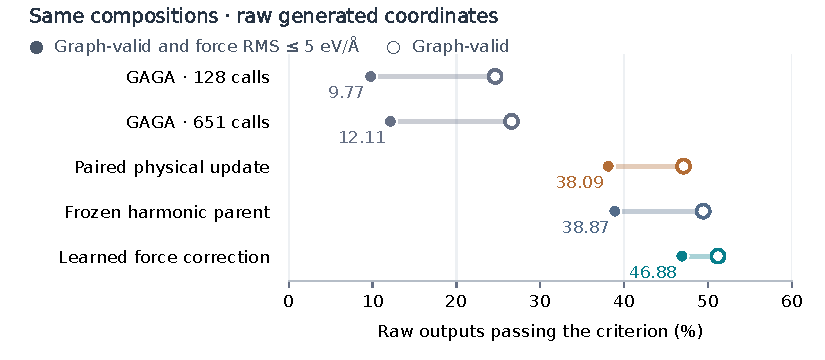
\includegraphics[width=\linewidth]{../research/figures/final_complete_v1/figures/common_model_quality.pdf}
\caption{Graph validity and joint yield on the common panel. Open circles show graph validity; filled circles also require GFN2 force RMS at most 5 eV/\AA. Connecting segments show the gap between the two criteria. Rates use all 512 attempts. Training histories and inference costs differ across systems, as described in the text.}
\label{fig:common-model-quality}
\end{figure}

\begin{table}[htbp]
\centering\small
\caption{Common-panel results on raw coordinates. Force medians use each model's graph-valid outputs with successful GFN2 calculations; joint yield uses all attempts. ``Calls'' lists backbone and head evaluations separately.}
\begin{tabular}{lrrrr}
\toprule
Model & Calls & Graph (\%) & Force (eV/\AA) & Joint (\%)\\
\midrule
GAGA &128&24.61&5.408&9.77\\
GAGA, complete schedule &651&26.56&5.176&12.11\\
Paired physical update &128&47.07&3.581&38.09\\
Paired update, no terminal noise &128&46.88&2.929&40.04\\
Frozen harmonic parent &128+64&49.41&3.394&38.87\\
Small correction, 2,000 updates &128+64&50.00&3.077&43.16\\
Small correction, 20,000 updates &128+64&51.17&2.854&46.88\\
Wide correction, 20,000 updates &128+64&50.20&2.831&46.09\\
Contextual correction, 20,000 updates &128+64&50.78&2.864&46.68\\
\bottomrule
\end{tabular}\label{tab:common-models}
\end{table}

The prespecified contextual head improves joint yield over its parent by 7.81 points (95\% interval $[4.88,10.94]$), with gains of 7.03 and 8.59 across fits. Its differences from the small and wide 20,000-update heads are $-0.20$ ($[-1.95,1.56]$) and $+0.59$ ($[-1.17,2.34]$). Thus lower internal target error does not yield a resolved advantage over the simpler heads.

The contextual system exceeds GAGA at 128 and 651 calls by 36.91 points ($[26.56,46.09]$) and 34.57 ($[24.80,43.95]$). The paired-update system exceeds them by 28.32 ($[20.70,35.74]$) and 25.98 ($[18.75,33.40]$). Appendices~\ref{app:feedback-transfer} and~\ref{app:matched-connection} provide architecture-controlled comparisons: both EGNN generators benefit from equal physical supervision, without a resolved ordering between them.

\paragraph{Terminal noise and fitting duration.}
The original-model and terminal-noise controls were specified before examining the new GFN2 results. We capture the zero-noise output from the same trajectory before the final 0.025\,\AA\ perturbation. Removing this noise adds 1.95 joint-yield points ($[0.39,3.71]$). The small head exceeds the paired-update model by 8.79 points ($[3.91,13.67]$) and its zero-noise variant by 6.84 ($[1.95,11.72]$), although their physical-training sets and parent histories differ.

A later duration diagnostic reuses the saved 2,000-update prefixes of the small-head fits. Targets, initialization, training states, and sampling match the 20,000-update versions. Longer fitting adds 3.71 points ($[1.76,5.86]$), with both fits improving. This comparison was added after inspecting the confirmation panel.

The small 20,000-update head also lowers all-output GFN2 energy relative to its parent by 0.0951 eV/atom (signed-change 95\% interval $[-0.2022,-0.0364]$), with reductions in both runs. The paired averages include invalid outputs and different connectivities.

\paragraph{Graph diagnostics and cost.}
Requiring zero assigned radical electrons gives joint yields of 46.29\% for the small head, 46.09\% for the contextual head, and 9.57\%/11.52\% for GAGA at its two budgets. No graph-valid output duplicates another inferred connectivity within a 16-draw composition/run cell; this measures observed duplication rather than isomer coverage.

The six-system confirmation uses 3,072 trajectories and GFN2 readouts. The parameter-matched control adds 40,000 head updates, following 80,000 updates in the earlier capacity study. Supplemental original-model and short-fit comparisons add 1,024 trajectories, 512 shared-trajectory noise variants, and 1,536 GFN2 readouts. All reuse the physical teacher and evaluate unoptimized coordinates.
